\subsection{Caso d'uso UC7: Compilazione questionario selezionato}
\begin{center}
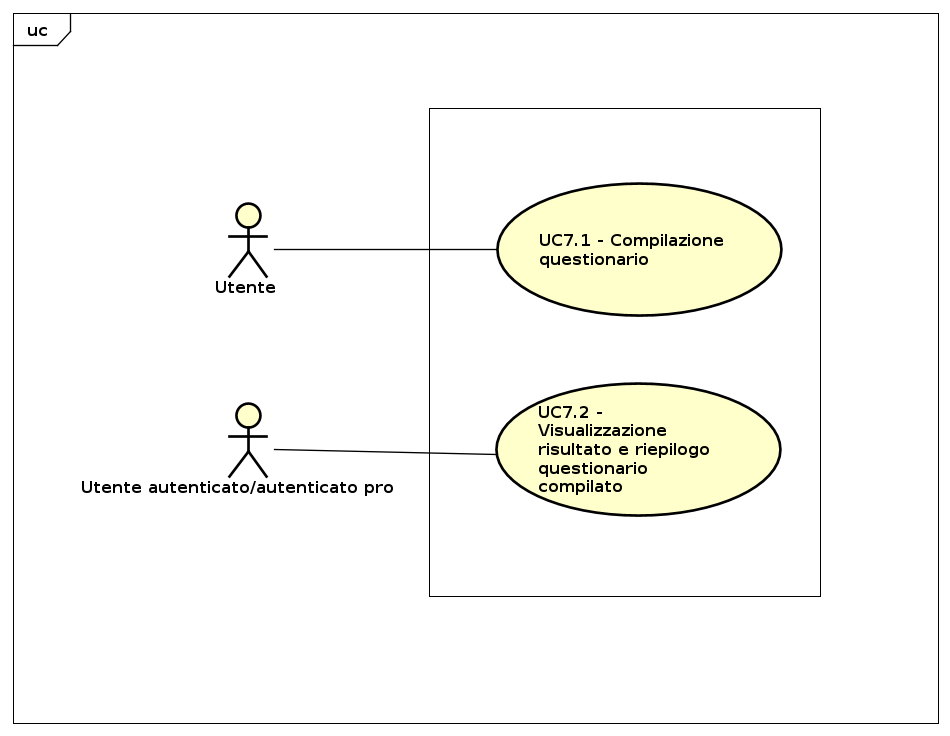
\includegraphics[scale=0.5]{UML/UC7.png}
\end{center}
\begin{itemize}
\item\textbf{Attori Principali}: Utente non autenticato, Utente autenticato, Utente autenticato pro;
\item\textbf{Descrizione}: l'utente autenticato/autenticato pro può compilare qualsiasi tipo di questionario e infine visualizzare il risultato ottenuto e il riepilogo delle risposte date. L'utente non autenticato invece può soltanto svolgere i questionari \textit{pubblici}.
\item\textbf{Precondizione}: l'utente ha selezionato un questionario;
\item\textbf{Postcondizione}: l'utente ha finito di compilare il questionario e può quindi visualizzare la valutazione finale che ha ottenuto e il riepilogo delle risposte date, se è un utente autenticato/autenticato pro;
\item\textbf{Scenario principale}:
\begin{itemize}
\item L'utente compila un questionario \textit{pubblico} (UC7.1);
\item L'utente autenticato/autenticato pro compila un questionario \textit{privato} (UC7.2);
\item L'utente autenticato/autenticato pro visualizza il risultato del questionario svolto (UC7.3).
\end{itemize}
\end{itemize}

\subsection{Caso d'uso UC7.1: Compilazione questionario pubblico}
\begin{itemize}
\item\textbf{Attori Principali}: Utente non autenticato, Utente autenticato, Utente autenticato pro;
\item\textbf{Descrizione}: -IDEA-: l'utente risponde alle domande che gli si presentano nell'ordine che preferisce spostandosi alla domanda successiva o a quella precedente ed infine conferma le risposte date;
\item\textbf{Precondizione}: l'utente ha selezionato un questionario \textit{pubblico};
\item\textbf{Postcondizione}: l'utente ha finito di compilare il questionario;
\item\textbf{Scenario principale}: -IDEA-:
\begin{itemize}
\item L'utente risponde ad una domanda (UC7.1.1);
\item L'utente passa alla domanda successiva (UC7.1.2);
\item L'utente passa alla domanda precedente (UC7.1.3);
\item L'utente conferma le risposte date alle domande (UC7.1.4);
\end{itemize}
\end{itemize}

\subsection{Caso d'uso UC7.2: Compilazione questionario privato}
\begin{center}
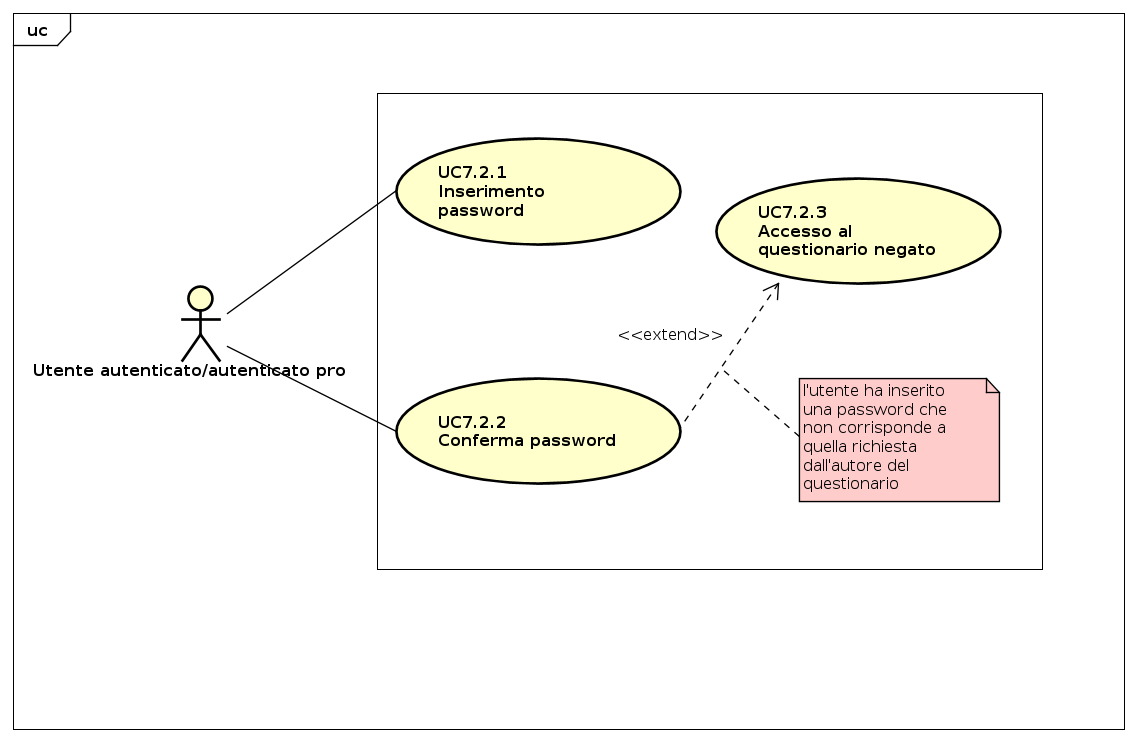
\includegraphics[scale=0.5]{UML/UC7_2.png}
\end{center}
\begin{itemize}
\item\textbf{Attori Principali}: Utente autenticato, Utente autenticato pro;
\item\textbf{Descrizione}: l'utente deve inserire la password richiesta dall'autore del questionario \textit{privato} e successivamente confermarla per poterlo compilare;
\item\textbf{Precondizione}: l'utente ha selezionato un questionario \textit{privato};
\item\textbf{Postcondizione}: l'utente ha finito di compilare il questionario;
\item\textbf{Scenario principale}:
\begin{itemize}
\item L'utente inserisce la password (UC7.2.1).
\item L'utente conferma l'inserimento della password (UC7.2.2)
\item L'utente compila il questionario (come in UC7.1)
\end{itemize}
\item\textbf{Scenario alternativo}: L'utente inserisce una password errata;
\item\textbf{Estensioni}: Accesso al questionario negato (UC7.2.3)
\end{itemize}

\subsection{Caso d'uso UC7.2.1: Inserimento password}
\begin{itemize}
\item\textbf{Attori Principali}: Utente autenticato, Utente autenticato pro;
\item\textbf{Descrizione}: l'utente per poter compilare il questionario deve inserire la password richiesta dal creatore di quest'ultimo;
\item\textbf{Precondizione}: l'utente ha selezionato un questionario \textit{privato};
\item\textbf{Postcondizione}: l'utente ha inserito la password;
\item\textbf{Scenario principale}: l'utente inserisce la password che gli consente di accedere al questionario.
\end{itemize}

\subsection{Caso d'uso UC7.2.2: Conferma password}
\begin{itemize}
\item\textbf{Attori Principali}: Utente autenticato, Utente autenticato pro;
\item\textbf{Descrizione}: l'utente conferma la password inserita per poter accedere al questionario;
\item\textbf{Precondizione}: l'utente ha inserito la password;
\item\textbf{Postcondizione}: l'utente ha confermato la password inserita;
\item\textbf{Scenario principale}: l'utente conferma la password.
\end{itemize}

\subsection{Caso d'uso UC7.2.3: Accesso al questionario negato}
\begin{itemize}
\item\textbf{Attori Principali}: Utente autenticato, Utente autenticato pro;
\item\textbf{Descrizione}: l'utente ha inserito una password che non corrisponde a quella richiesta dall'autore del questionario, generando così un errore che gli impedirà di proseguire con la compilazione del suddetto fino a quando non inserirà la password corretta;
\item\textbf{Precondizione}: l'utente ha provato a confermare una password errata;
\item\textbf{Postcondizione}: il sistema avvisa l'utente dell'errore verificatosi tramite un opportuno messaggio;
\item\textbf{Scenario principale}: l'utente visualizza il messaggio di errore relativo alla password scorretta.
\end{itemize}

\subsection{Caso d'uso UC7.3: Visualizzazione risultato questionario compilato}
\begin{itemize}
\item\textbf{Attori Principali}: Utente autenticato, Utente autenticato pro;
\item\textbf{Descrizione}: l'utente, dopo aver finito di compilare il questionario, visualizzerà una schermata contenente il riepilogo delle risposte date alle domande. Sarà possibile vedere quali di queste sono corrette e quali no e verrà inoltre data una valutazione complessiva;
\item\textbf{Precondizione}: l'utente ha finito di compilare il questionario che ha scelto di affrontare;
\item\textbf{Postcondizione}: il sistema visualizza una schermata contenente il riepilogo del questionario svolto e un voto;
\item\textbf{Scenario principale}: L'utente visualizza che voto gli è stato dato e quali domande ha sbagliato.
\end{itemize}

